%
%	Section 3: The Mbrace runtime
%

\section{The \TitularMbrace{} Distributed Runtime}
\label{sec:runtime}

The \mbrace{} runtime is the execution environment of the \mbrace{} framework
that implements the execution semantics of cloud workflows and cloud data
as described previously. A typical \mbrace{} runtime instance comprises
multiple nodes forming a cluster. The runtime is responsible for executing cloud
workflows, managing and monitoring the nodes and resources within a cluster,
elasticity, fault tolerance and integration with distributed storage providers.

From a user's perspective the \mbrace{} runtime provides an abstraction over a
cluster analogous to that of an operating system over hardware. A cloud
workflow, representing a deferred computation as described earlier, along with
any code and dependencies effectively forms the cloud program executable by the
runtime, of which an executing instance is a \emph{cloud process}. Multiple
cloud processes are executed concurrently and in isolation in the much the same
sense as in traditional multi-process operating systems. The runtime monitors
and manages the computational and data resources available within the cluster,
which are allocated between cloud processes based on load and runtime
statistics.
%
\begin{figure}[ht]
\label{runtime-figure}
\centering
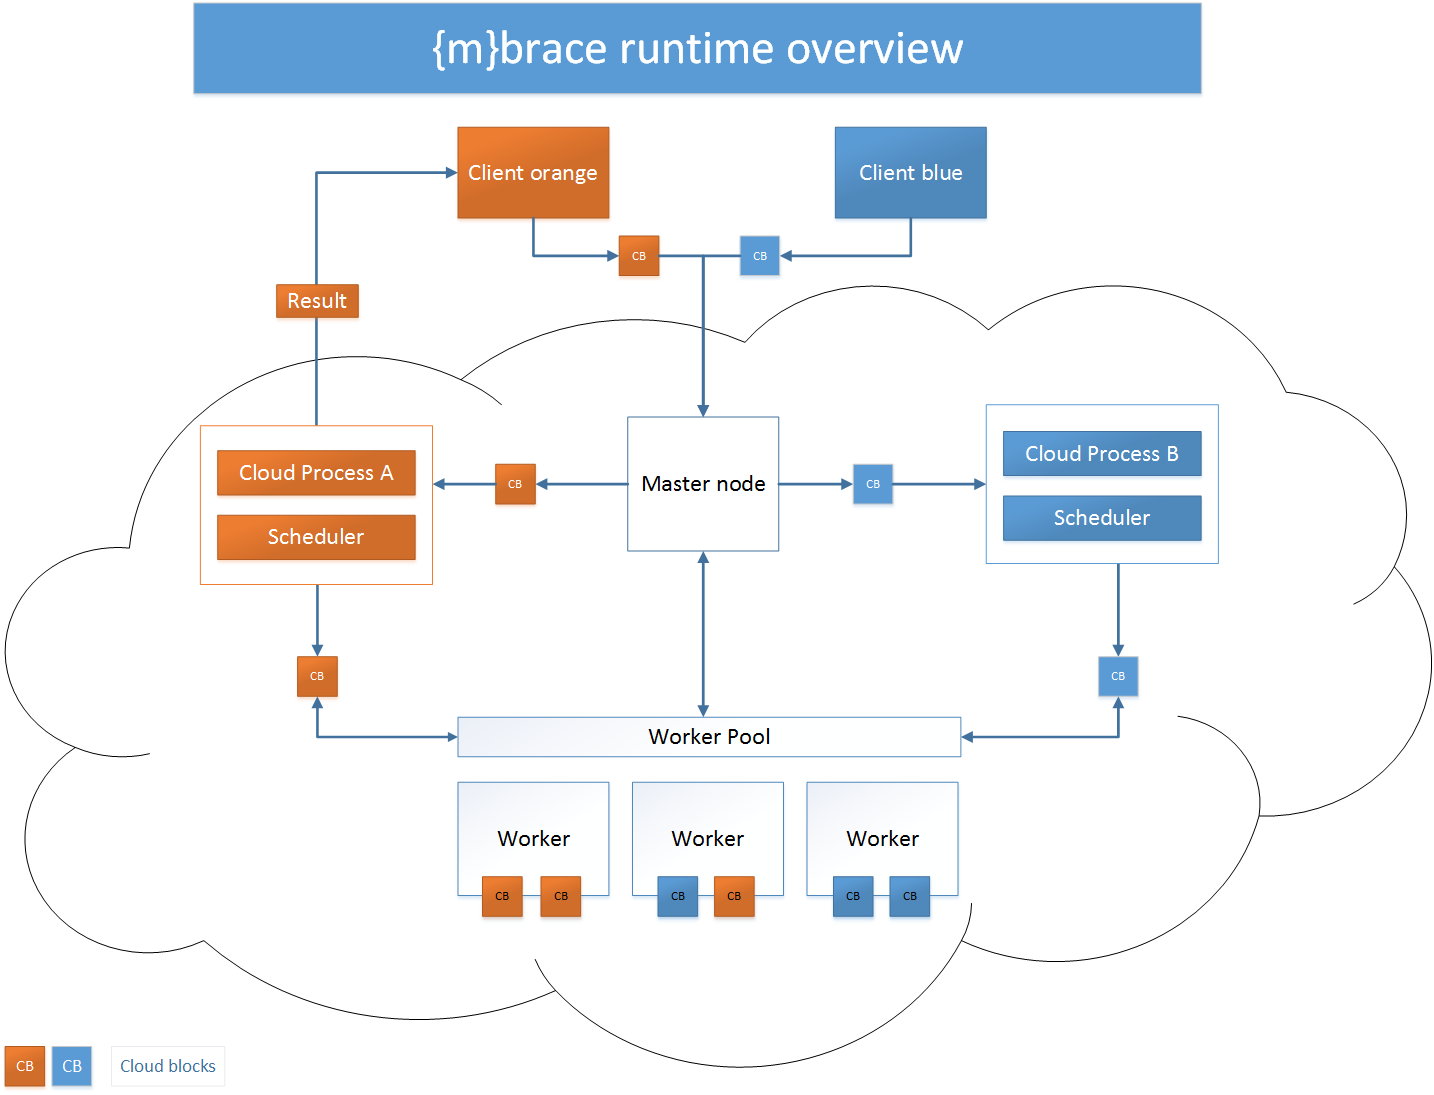
\includegraphics[width=0.8\textwidth]{runtime.png}
\caption{Architectural overview of the \mbrace{} runtime.}
\end{figure}

In figure \ref{runtime-figure} we give an architectural overview of a \mbrace{}
cluster instance. Each cluster instance has a unique \emph{master node} which is
responsible for monitoring the health of the nodes participating in the cluster
as well as gathering other runtime statics, such as CPU and network loads. All
other nodes are slave nodes. A subset of slave nodes are \emph{alternative
  masters}. Alternative master nodes replicate the master node's state. In the
event of a master node failure, a new master node will be selected from the
available alternatives while a slave node will be added to the alternative set.

The execution of a cloud process employs a \emph{scheduler-worker} scheme. One
node is selected to be the process scheduler with the rest being worker
nodes. The scheduler unfolds the cloud workflow in execution and allocates
pending jobs to available workers. Scheduling is load balanced taking into
account relevant runtime statics such as CPU and network load of the available
workers. The scheduler maintains state tracking the job allocation, which is
replicated between a subset of the available worker nodes. In the event of a
worker node failure this allows the scheduler to re-schedule any lost jobs,
while in the event of the scheduler node failure a new scheduler is selected
from the available worker nodes and its state is re-applied.

Cluster nodes are shared between concurrently executing cloud
processes. However, the runtime enforces an \emph{isolation} policy where each
cloud process is allocated a distinct CLI instance in each node. The set of all
CLI instances allocated to a cloud process is the unit isolation and is called a
\emph{process domain}. Each cloud process inhibits a distinct process
domain. Thus a single cluster node may host multiple CLI scheduler and worker
instances from different cloud processes. This enables a more robust runtime as
local process failures are isolated and leads to more efficient memory
management as each CLI instance has its own garbage collector. Note that each
cloud process is allocated its own scheduler offering a further level of
isolation in terms of scheduling load. Again, allocating schedulers to cloud
processes is balanced between the available nodes.

Finally, the \mbrace{} runtime offers pluggable support for a range of
distributed store providers. Storage providers are essential for a runtime to
function, since they are used for internal caching and make possible the
definition of cloud refs. \mbrace{} comes with support for FileSystem, SQL and
Azure storage providers, while providing user-defined custom implementations is
also possible.

\subsection{The \TitularMbrace{} Daemon}

As mentioned earlier, the \mbrace{} daemon is the server-side application that
bootstraps a machine-wide instance of the \mbrace{} framework. It is initialized by
running the \texttt{mbraced.exe} executable, typically found in the binaries
folder of every \mbrace{} installation. For instance, the command
\begin{verbatim}
   $ mbraced.exe --hostname 127.0.0.1 --primary-port 2675 --detach
\end{verbatim}
will instantiate a background \texttt{mbraced} process that listens on
the loopback interface at port 2675.

\subsubsection*{Configuring the \TitularMbrace{} Daemon}

The \mbrace{} daemon comes with a range of configuration options.
These parameters can either be read from the \texttt{mbraced} configuration file, 
or passed as command line arguments, in that evaluation order.
Command line parameters override those provided by the configuration file.

As is common in \dotnet{} applications, \texttt{mbraced} comes with an xml
configuration file, namely \texttt{mbraced.exe.config} found in the same location 
as the executable. Configuration for \texttt{mbraced} is written in the 
\texttt{AppSettings} section of the xml document that follows a key-value 
schema:
\begin{lstlisting}[language=Xml]
<?xml version="1.0" encoding="utf-8"?>
<configuration>
  <appSettings>
    <add key="hostname" value="grothendieck.nessos"/>
    <add key="primary port" value="2675"/>
    <add key="worker port range" value="30000, 30042"/>
    <add key="working directory" value="/var/mbraced/"/>
    <add key="log file" value="mbrace-log.txt"/>
    <!-- specify loglevel: info 0, warning 1, error 2-->
    <add key="log level" value="0"/>
    <!-- executable name of mbrace child process -->
    <add key="mbrace processdomain executable" value="mbrace.worker.exe"/>
  </appSettings>
</configuration>
\end{lstlisting}
The full range of command line parameters for \texttt{mbraced} can be viewed by typing
\begin{verbatim}
   $ mbraced.exe --help
\end{verbatim}
%
We now give a brief description of the configuration parameters offered by the daemon:
\begin{description}[style=unboxed, font=\sffamily]
\item[Hostname] The ip address or host name that the daemon listens to.
The hostname must be resolvable in the context of the entire \mbrace{} cluster.
Each instance of \texttt{mbraced} can only have one hostname specified.
\item[Primary Port] The tcp port that the local cluster supervisor listens to.
\item[Worker Port Range] A range or collection of tcp ports that can be assigned
to worker processes spawned by the local cluster supervisor.
\item[Working Directory] The local directory in which all local caching is performed.
Write permissions are required for the daemon process.
\item[Log File] Specifies the path to the log file. If relative, it is resolved with
respect to the working directory.
\item[Log Level] Specifies the log level: 0 for info, 1 for warnings, 2 for errors.
\item[ProcessDomain Executable] The location of the worker process executable.
Relative paths evaluated with respect to the main \texttt{mbraced.exe} path.
\end{description}

\subsubsection*{Deploying the \TitularMbrace{} Daemon}

Once the configuration file for \texttt{mbraced} has been set up as desired,
deploying an instance from the command line is as simple as typing
\begin{verbatim}
    $ mbraced --detach
\end{verbatim}
The \mbrace{} framework also comes with the \texttt{mbracectl} command line tool
that can be used to track deployment state. Initiating a session can be done like so:
\begin{verbatim}
    $ mbracectl start
\end{verbatim}
This will initialize a background instance with settings read from the \texttt{mbraced}
configuration file. Session state can be queried by entering
\begin{verbatim}
    $ mbracectl status
\end{verbatim}
Finally, a session can be ended by typing
\begin{verbatim}
    $ mbracectl stop
\end{verbatim}
\texttt{mbracectl} can also be used to initiate multiple instances on the local machine
\begin{verbatim}
    $ mbracectl start --nodes 16 --spawn-window
\end{verbatim}
that can even be booted in a local cluster
\begin{verbatim}
    $ mbracectl start --nodes 3 --boot
\end{verbatim}

The \mbrace{} installer also comes bundled with a windows service.
Initiating \texttt{mbraced} as a service will spawn a background instance
with settings read from the xml configuration file.

Once the required \texttt{mbraced} instances have been deployed as desired,
they can be reached from the client API as seen in section \ref{sec:client}
using the \texttt{mbrace} connection string.


%%% Local Variables: 
%%% mode: latex
%%% TeX-master: "mbrace"
%%% End: 
